\documentclass[a4paper,11pt]{article}
\usepackage[utf8]{inputenc}
\usepackage[T1]{fontenc}
\usepackage{amsmath,amssymb}
\usepackage[a4paper,left=2cm,right=2cm,top=3.6cm,bottom=2.3cm,headheight=1.1cm,headsep=0.6cm,footskip=1cm]{geometry}
\usepackage{xcolor}
\usepackage{tikz}
\usetikzlibrary{calc,arrows.meta,positioning,shapes.geometric,matrix}
\usepackage{fancyhdr}
\usepackage{lastpage}
\usepackage{tabularx}
\usepackage{array}
\usepackage[most]{tcolorbox}
\usepackage{enumitem}
\usepackage{needspace}

% ---------- palet sky (Sky-800 dan Sky-200) ----------
\definecolor{mainc}{HTML}{075985}
\definecolor{accc}{HTML}{0284C7}
\definecolor{skyl}{HTML}{BAE6FD}
\definecolor{deepc}{HTML}{082F49}
\definecolor{softbg}{HTML}{F0F9FF}
\definecolor{warmc}{HTML}{D97706}
\definecolor{brick}{HTML}{B91C1C}
\newcommand{\dis}{\displaystyle}
\newcommand{\Pm}[2]{{}_{#1}P_{#2}}

\setlength{\parindent}{0pt}
\renewcommand{\arraystretch}{1.35}

\tikzset{
  ar/.style={-{Stealth[length=1.8mm]},thick,mainc},
  box/.style={draw=mainc,thick,rounded corners=3pt,fill=softbg,align=center,inner sep=4pt},
  nd/.style={circle,draw=mainc,thick,fill=softbg,minimum size=6mm,inner sep=0pt,font=\scriptsize}
}

% ---------- header ----------
\pagestyle{fancy}
\fancyhf{}
\renewcommand{\headrulewidth}{0pt}
\fancyhead[L]{%
  \begin{tikzpicture}[remember picture,overlay]
    \fill[mainc] ([yshift=-1.2cm]current page.north west) rectangle ([yshift=-3.15cm]current page.north east);
    \fill[skyl] ([yshift=-3.15cm]current page.north west) rectangle ([yshift=-3.3cm]current page.north east);
  \end{tikzpicture}%
  \color{white}\bfseries\large Latihan Soal Analisis Data dan Peluang}
\fancyhead[R]{\color{white}\small Diunduh dari website \textbf{Math1729}\ \,|\,\ 5 Oktober 2026}
\fancyfoot[L]{\small\color{mainc}Math1729 --- Analisis Data dan Peluang}
\fancyfoot[R]{\small\color{mainc}Halaman \thepage\ dari \pageref{LastPage}}

% ---------- komponen ----------
\newcounter{no}
\newcommand{\bagian}[2]{\par\Needspace{6\baselineskip}\vspace{1.0em}\noindent
  \begin{tcolorbox}[colback=mainc,colframe=mainc,coltext=white,boxrule=0pt,arc=2pt,left=6pt,right=6pt,top=3pt,bottom=3pt]
  \textbf{#1}\hfill{\small #2}\end{tcolorbox}\setcounter{no}{0}\par\vspace{-0.3em}}
\newcommand{\tingkat}[2]{\par\Needspace{7\baselineskip}\vspace{0.6em}\noindent
  {\color{accc}\rule{3pt}{1.1em}}\ {\color{mainc}\bfseries #1}\ {\small\color{gray}--- #2}\par\vspace{0.1em}}
\newcommand{\soal}[2]{\par\vspace{0.75em}\stepcounter{no}\noindent
  \begin{minipage}[t]{1.8em}\textbf{\theno.}\end{minipage}%
  \begin{minipage}[t]{\dimexpr\linewidth-1.8em\relax}#1\par\vspace{0.35em}#2\end{minipage}\par}
\newcommand{\poin}[1]{\hfill{\small\color{mainc}[#1 poin]}}
\newcommand{\gbr}[2]{\noindent\begin{minipage}[t]{0.56\linewidth}#1\end{minipage}\hfill\raisebox{\ht\strutbox}{\begin{minipage}[t]{0.41\linewidth}\vspace{0pt}\centering#2\end{minipage}}}
\newcommand{\pil}[5]{\begin{tabularx}{\linewidth}{@{}*{5}{X}@{}}\textbf{A.}\;#1 & \textbf{B.}\;#2 & \textbf{C.}\;#3 & \textbf{D.}\;#4 & \textbf{E.}\;#5\end{tabularx}}
\newcommand{\pilx}[5]{\begin{tabularx}{\linewidth}{@{}*{3}{X}@{}}\textbf{A.}\;#1 & \textbf{B.}\;#2 & \textbf{C.}\;#3\\[10pt] \textbf{D.}\;#4 & \textbf{E.}\;#5 & \end{tabularx}}
\newcommand{\jwb}{\hfill Jawaban: \rule{4.5cm}{0.4pt}}

% ---------- tambahan khusus materi ini ----------
\newcommand{\Var}{\operatorname{Var}}
\pgfmathdeclarefunction{bell}{1}{\pgfmathparse{2.4*exp(-(#1)*(#1)/2)}}
\newcommand{\shadearea}[3]{\fill[#1] (#2,0) -- plot[domain=#2:#3,samples=50] (\x,{bell(\x)}) -- (#3,0) -- cycle;}
\newcommand{\bellcurve}{\draw[very thick,mainc,domain=-3.4:3.4,samples=70] plot (\x,{bell(\x)});\draw[thick,mainc] (-3.5,0)--(3.5,0);}

\begin{document}
\thispagestyle{fancy}

\begin{center}
  {\color{mainc}\fontsize{22}{26}\selectfont\bfseries Latihan Soal Analisis Data dan Peluang\par}
  \vspace{2pt}
  {\color{accc}\large Variabel Acak, Distribusi Seragam, Binomial, Normal, dan Penalaran Data\par}
\end{center}
\vspace{2pt}
\begin{tcolorbox}[colback=softbg,colframe=mainc!40,boxrule=0.6pt,arc=3pt,left=8pt,right=8pt,top=5pt,bottom=5pt]
\noindent\textbf{Nama} : \rule{4.6cm}{0.4pt}\hfill\textbf{Kelas} : \rule{2.2cm}{0.4pt}\hfill\textbf{Skor} : \rule{2.2cm}{0.4pt}
\end{tcolorbox}
\vspace{2pt}
\begin{tcolorbox}[colback=white,colframe=accc,boxrule=0.8pt,arc=3pt,left=8pt,right=8pt,top=4pt,bottom=4pt,title={\bfseries Petunjuk Pengerjaan},coltitle=white,fonttitle=\small]
\small
\begin{enumerate}[leftmargin=1.4em,itemsep=1pt,topsep=1pt]
\item Soal terdiri atas \textbf{20 pilihan ganda} (5 mudah, 6 sedang, 8 sulit, 1 HOTS), \textbf{5 isian singkat} (2 sedang, 3 sulit), dan \textbf{5 uraian (essay)} (2 sedang, 2 sulit, 1 HOTS). Soal disusun berjenjang dan memakai bentuk yang sejalan dengan UTBK-SNBT 2026, yang menilai penalaran matematika melalui tiga proses: \emph{merumuskan} masalah dari konteks, \emph{menggunakan} konsep dan prosedur, serta \emph{menafsirkan} hasilnya. Bentuk yang dipakai: pilihan ganda lima opsi, pilihan majemuk kompleks (benar/salah), kecukupan data, soal konteks yang menyajikan data lewat gambar, grafik, atau tabel, isian singkat, dan uraian bertahap. Alokasi waktu yang disarankan: 120 menit.
\item Skor: pilihan ganda 2 poin, isian singkat 4 poin, uraian 8 poin per soal (total 100 poin). Tidak ada pengurangan skor untuk jawaban salah.
\item Notasi: $X\sim U(a,b)$ distribusi seragam, $X\sim B(n,p)$ distribusi binomial, $X\sim N(\mu,\sigma^2)$ distribusi normal, $\Var(X)$ variansi, dan $\Phi(z)=P(Z\le z)$ untuk $Z\sim N(0,1)$ dengan $\Phi(-z)=1-\Phi(z)$. Aturan empiris: $68\%$, $95\%$, $99{,}7\%$ untuk $\mu\pm\sigma$, $\mu\pm2\sigma$, $\mu\pm3\sigma$. Tabel yang boleh dipakai:
\begin{center}\small\renewcommand{\arraystretch}{1.2}
\begin{tabular}{|c|c|c|c|c|c|c|}\hline
$z$ & $0{,}5$ & $1{,}0$ & $1{,}5$ & $2{,}0$ & $2{,}5$ & $3{,}0$\\\hline
$\Phi(z)$ & $0{,}6915$ & $0{,}8413$ & $0{,}9332$ & $0{,}9772$ & $0{,}9938$ & $0{,}9987$\\\hline
\end{tabular}\end{center}
\item Bilangan ribuan ditulis dengan tanda titik dan bilangan desimal dengan tanda koma. Gambar tidak selalu digambar sesuai skala. Pada isian singkat, tuliskan hanya jawaban akhir.
\item Kalkulator tidak diperkenankan. Hasil boleh berupa pecahan paling sederhana atau desimal sesuai perintah soal.
\end{enumerate}
\end{tcolorbox}

% =====================================================================
\bagian{A. Pilihan Ganda}{20 soal $\times$ 2 poin = 40 poin. Pilih satu jawaban yang paling tepat.}

\tingkat{Tingkat Mudah}{soal 1 sampai 5}
\soal{\gbr{Diagram batang berikut menyajikan distribusi peluang variabel acak diskret $X$. Peluang $P(X=2)=k$ belum diketahui. Nilai harapan $E(X)$ adalah \dots.}{%
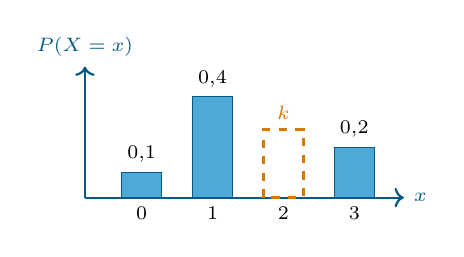
\begin{tikzpicture}[x=0.9cm,y=3.2cm]
\draw[->,thick,mainc] (0.2,0)--(4.7,0) node[right,font=\scriptsize]{$x$};
\draw[->,thick,mainc] (0.2,0)--(0.2,0.52) node[above,font=\scriptsize]{$P(X=x)$};
\foreach \cx/\hh/\lab/\val in {1/0.1/0/{0{,}1},2/0.4/1/{0{,}4},4/0.2/3/{0{,}2}}{
 \fill[accc!70] (\cx-0.28,0) rectangle (\cx+0.28,\hh);
 \draw[mainc] (\cx-0.28,0) rectangle (\cx+0.28,\hh);
 \node[font=\scriptsize,above] at (\cx,\hh) {$\val$};
 \node[font=\scriptsize,below] at (\cx,0) {$\lab$};}
\draw[warmc,very thick,dashed] (2.72,0) rectangle (3.28,0.27);
\node[font=\scriptsize\bfseries,warmc,above] at (3,0.27) {$k$};
\node[font=\scriptsize,below] at (3,0) {$2$};
\end{tikzpicture}}}{\pil{$1{,}0$}{$1{,}6$}{$1{,}8$}{$2{,}0$}{$2{,}2$}}
\soal{Nomor antrean $1$ sampai $40$ dibagikan kepada pengunjung sebuah klinik. Satu nomor dipilih secara acak untuk mendapat suvenir. Peluang nomor yang terpilih adalah \textbf{kelipatan $6$ atau kelipatan $8$} adalah \dots.}{\pil{$\dfrac3{20}$}{$\dfrac15$}{$\dfrac9{40}$}{$\dfrac14$}{$\dfrac{11}{40}$}}
\soal{Seorang kiper menahan tendangan penalti dengan peluang $0{,}7$. Dari tiga tendangan penalti berurutan yang hasilnya saling bebas, peluang kiper menahan \textbf{tepat dua} tendangan adalah \dots.}{\pil{$0{,}189$}{$0{,}343$}{$0{,}441$}{$0{,}784$}{$0{,}973$}}
\soal{\gbr{Waktu tempuh sebuah bus dari terminal ke kampus berdistribusi normal dengan rata-rata $30$ menit dan simpangan baku $2$ menit (lihat gambar). Berdasarkan aturan empiris, persentase perjalanan yang waktunya \textbf{kurang dari $26$ menit} adalah \dots.}{%
\begin{tikzpicture}[x=0.55cm,y=0.6cm]
\shadearea{warmc!55}{-3.4}{-2}
\bellcurve
\draw[dashed,mainc] (-2,0)--(-2,{bell(-2)});
\node[font=\scriptsize,below] at (0,0) {30};
\node[font=\scriptsize\bfseries,warmc!70!black,below] at (-2,0) {26};
\node[font=\scriptsize,mainc] at (0,0.7) {menit};
\end{tikzpicture}}}{\pil{$2{,}5\%$}{$5\%$}{$16\%$}{$34\%$}{$68\%$}}
\soal{Tentukan nilai kebenaran tiga pernyataan berikut (B = benar, S = salah), berurutan dari (i) sampai (iii).\par\smallskip
(i) Pada distribusi normal, rata-rata, median, dan modus bernilai sama.\par
(ii) Jika $X\sim B(10;0{,}3)$, maka $E(X)=3$ dan $\Var(X)=2{,}1$.\par
(iii) Jika $X\sim U(0,10)$ kontinu, maka $P(X=5)=\dfrac1{10}$.}{\pilx{S, S, S}{B, S, B}{S, B, B}{B, B, B}{B, B, S}}

\tingkat{Tingkat Sedang}{soal 6 sampai 11}
\soal{\gbr{Lampu lalu lintas menyala merah selama $120$ detik. Seorang pengendara tiba di persimpangan secara acak saat lampu merah, sehingga sisa waktu merah $X$ (dalam detik) berdistribusi seragam kontinu seperti pada grafik. Diketahui sisa waktu merah \textbf{lebih dari $30$ detik}. Peluang sisa waktu merah \textbf{paling lama $90$ detik} adalah \dots.}{%
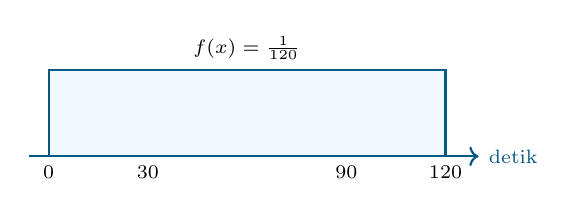
\begin{tikzpicture}[x=0.042cm,y=1cm]
\draw[->,thick,mainc] (-6,0)--(130,0) node[right,font=\scriptsize]{detik};
\fill[softbg] (0,0) rectangle (120,1.1);
\draw[mainc,thick] (0,0) rectangle (120,1.1);
\foreach \q in {0,30,90,120}{\node[font=\scriptsize,below] at (\q,0) {$\q$};}
\node[font=\scriptsize,above] at (60,1.1) {$f(x)=\frac1{120}$};
\end{tikzpicture}}}{\pil{$\dfrac13$}{$\dfrac12$}{$\dfrac35$}{$\dfrac23$}{$\dfrac34$}}
\soal{Dalam satu pengiriman terdapat $4$ komponen elektronik yang diuji secara terpisah. Setiap komponen lolos uji dengan peluang $0{,}8$. Peluang \textbf{paling banyak dua} komponen yang lolos uji adalah \dots.}{\pil{$0{,}1808$}{$0{,}4096$}{$0{,}5904$}{$0{,}8192$}{$0{,}9728$}}
\soal{Skor sebuah tes berdistribusi normal. Rina memperoleh skor $78$, yaitu $1{,}5$ simpangan baku di atas rata-rata, sedangkan Dani memperoleh skor $66$, yaitu $0{,}5$ simpangan baku di bawah rata-rata. Peluang seorang peserta memperoleh skor \textbf{lebih dari $75$} adalah \dots.}{\pil{$0{,}1587$}{$0{,}3085$}{$0{,}6915$}{$0{,}8413$}{$0{,}9332$}}
\soal{\gbr{Grafik tangga di samping adalah fungsi distribusi kumulatif $F(x)=P(X\le x)$ dari variabel acak diskret $X$ yang bernilai $0,1,2,3$. Nilai harapan $E(X)$ adalah \dots.}{%
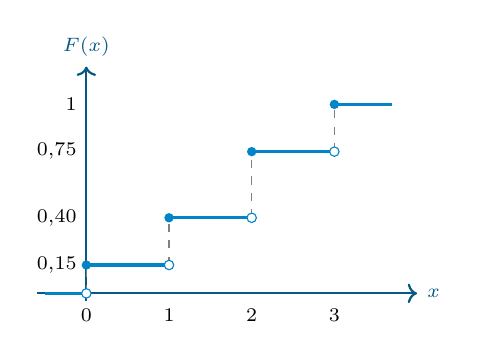
\begin{tikzpicture}[x=1.05cm,y=2.4cm]
\draw[->,thick,mainc] (-0.6,0)--(4.0,0) node[right,font=\scriptsize]{$x$};
\draw[->,thick,mainc] (0,-0.04)--(0,1.2) node[above,font=\scriptsize]{$F(x)$};
\draw[accc,very thick] (-0.5,0)--(0,0) (0,0.15)--(1,0.15) (1,0.40)--(2,0.40) (2,0.75)--(3,0.75) (3,1)--(3.7,1);
\draw[gray,dashed] (1,0.15)--(1,0.40) (2,0.40)--(2,0.75) (3,0.75)--(3,1) (0,0)--(0,0.15);
\foreach \ix/\iy in {0/0.15,1/0.40,2/0.75,3/1}{\fill[accc] (\ix,\iy) circle (1.7pt);}
\foreach \ix/\iy in {0/0,1/0.15,2/0.40,3/0.75}{\draw[accc,fill=white] (\ix,\iy) circle (1.7pt);}
\foreach \ix in {0,1,2,3}{\node[font=\scriptsize,below] at (\ix,-0.03) {$\ix$};}
\foreach \iy/\lab in {0.15/{0{,}15},0.40/{0{,}40},0.75/{0{,}75},1/{1}}{\node[font=\scriptsize,left] at (0,\iy) {$\lab$};}
\end{tikzpicture}}}{\pil{$1{,}40$}{$1{,}50$}{$1{,}55$}{$1{,}65$}{$1{,}70$}}
\soal{Variabel acak $X$ berdistribusi binomial $B(n,p)$. Nilai harapan $X$ sama dengan dua kali variansinya, dan $P(X=n)=\dfrac1{64}$. Nilai $P(X\ge5)$ adalah \dots.}{\pil{$\dfrac1{64}$}{$\dfrac7{64}$}{$\dfrac{15}{64}$}{$\dfrac{11}{32}$}{$\dfrac{21}{32}$}}
\soal{\gbr{Nilai ujian sekolah berdistribusi normal dengan rata-rata $72$ dan simpangan baku $8$. Siswa yang nilainya berada pada $6{,}68\%$ terbawah (daerah berarsir) wajib mengikuti remedial. Nilai terendah agar siswa \textbf{tidak} mengikuti remedial (nilai $k$ pada gambar) adalah \dots.}{%
\begin{tikzpicture}[x=0.55cm,y=0.6cm]
\shadearea{warmc!55}{-3.4}{-1.5}
\bellcurve
\draw[dashed,mainc] (-1.5,0)--(-1.5,{bell(-1.5)});
\node[font=\scriptsize,below] at (0,0) {72};
\node[font=\scriptsize\bfseries,warmc!70!black,below] at (-1.5,0) {$k$};
\node[font=\tiny,warmc!70!black] at (-2.7,0.8) {$6{,}68\%$};
\end{tikzpicture}}}{\pil{$48$}{$52$}{$56$}{$60$}{$84$}}

\tingkat{Tingkat Sulit}{soal 12 sampai 19, setara UTBK}
\soal{Dalam sebuah permainan, pemain melempar $4$ koin seimbang sekali. Jika muncul $X$ sisi gambar, pemain menerima hadiah $X^2$ ribu rupiah. Untuk satu kali bermain, pemain membayar Rp6.000. Dalam jangka panjang, hasil rata-rata pemain per permainan adalah \dots.}{\pilx{untung Rp1.000}{impas}{rugi Rp500}{rugi Rp2.000}{rugi Rp1.000}}
\soal{\gbr{Berat bersih sebungkus kopi berdistribusi normal. Diketahui $15{,}87\%$ bungkus beratnya kurang dari $40$ gram dan $2{,}28\%$ bungkus beratnya lebih dari $70$ gram (lihat gambar). Peluang berat sebungkus kopi \textbf{antara $45$ dan $65$ gram} adalah \dots.}{%
\begin{tikzpicture}[x=0.5cm,y=0.6cm]
\shadearea{warmc!55}{-3.4}{-1}
\shadearea{brick!45}{2}{3.4}
\bellcurve
\draw[dashed,mainc] (-1,0)--(-1,{bell(-1)}) (2,0)--(2,{bell(2)});
\node[font=\scriptsize\bfseries,below] at (-1,0) {40};
\node[font=\scriptsize\bfseries,below] at (2,0) {70};
\node[font=\scriptsize,below] at (0,0) {$\mu$};
\node[font=\tiny,warmc!70!black] at (-2.7,0.85) {$15{,}87\%$};
\node[font=\tiny,brick] at (3.0,0.85) {$2{,}28\%$};
\end{tikzpicture}}}{\pil{$0{,}2417$}{$0{,}6247$}{$0{,}6915$}{$0{,}8185$}{$0{,}9332$}}
\soal{\gbr{Variabel acak $X$ berdistribusi binomial $B(4,p)$. Pada diagram batang, hanya batang $X=0$ yang diberi nilai, yaitu $P(X=0)=\dfrac{16}{81}$ (tinggi batang lain sesuai skala). Peluang $X$ \textbf{paling banyak} $1$ adalah \dots.}{%
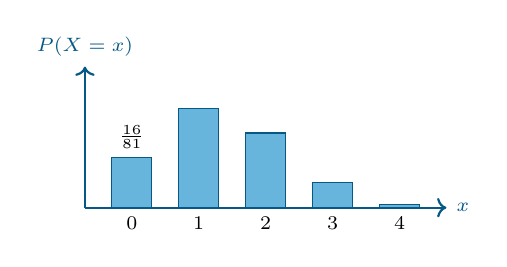
\begin{tikzpicture}[x=0.85cm,y=3.2cm]
\draw[->,thick,mainc] (-0.2,0)--(5.2,0) node[right,font=\scriptsize]{$x$};
\draw[->,thick,mainc] (-0.2,0)--(-0.2,0.56) node[above,font=\scriptsize]{$P(X=x)$};
\foreach \ix/\hh in {0/0.1975,1/0.3951,2/0.2963,3/0.0988,4/0.0123}{
 \fill[accc!60] (\ix+0.2,0) rectangle (\ix+0.8,\hh);
 \draw[mainc] (\ix+0.2,0) rectangle (\ix+0.8,\hh);
 \node[font=\scriptsize,below] at (\ix+0.5,0) {$\ix$};}
\node[font=\scriptsize,above] at (0.5,0.1975) {$\frac{16}{81}$};
\end{tikzpicture}}}{\pil{$\dfrac19$}{$\dfrac8{27}$}{$\dfrac{32}{81}$}{$\dfrac{11}{27}$}{$\dfrac{16}{27}$}}
\soal{Jika $X$ berdistribusi binomial $B(20;0{,}3)$, nilai $x$ yang membuat $P(X=x)$ paling besar adalah \dots.}{\pil{$3$}{$4$}{$5$}{$6$}{$7$}}
\soal{Lima koin seimbang dilempar bersamaan. Jika diketahui \textbf{paling sedikit satu} koin menunjukkan gambar, peluang bahwa \textbf{tepat dua} koin menunjukkan gambar adalah \dots.}{\pil{$\dfrac5{32}$}{$\dfrac5{16}$}{$\dfrac{10}{31}$}{$\dfrac13$}{$\dfrac58$}}
\soal{Nilai ujian $500$ siswa berdistribusi normal dengan rata-rata $60$ dan simpangan baku $12$. Agar sebarannya sesuai standar sekolah, setiap nilai $x$ diubah menjadi $y=ax+b$ dengan $a>0$ sehingga nilai baru memiliki rata-rata $70$ dan simpangan baku $9$. Banyak siswa yang nilai barunya \textbf{lebih dari $79$} kira-kira \dots.}{\pil{$8$}{$16$}{$79$}{$250$}{$421$}}
\soal{\gbr{Bilangan $X$ dipilih secara acak dari selang $[-3,6]$ dan berdistribusi seragam kontinu (lihat grafik). Peluang persamaan kuadrat $t^2-2Xt+(X+6)=0$ memiliki akar-akar real adalah \dots.}{%
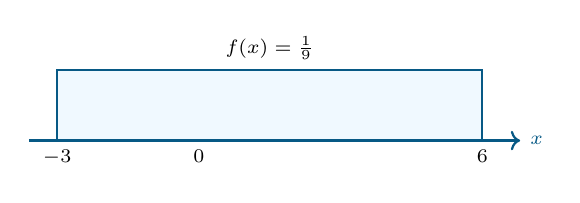
\begin{tikzpicture}[x=0.6cm,y=1cm]
\draw[->,thick,mainc] (-3.6,0)--(6.8,0) node[right,font=\scriptsize]{$x$};
\fill[softbg] (-3,0) rectangle (6,0.9);
\draw[mainc,thick] (-3,0) rectangle (6,0.9);
\foreach \q in {-3,0,6}{\node[font=\scriptsize,below] at (\q,0) {$\q$};}
\node[font=\scriptsize,above] at (1.5,0.9) {$f(x)=\frac19$};
\end{tikzpicture}}}{\pil{$\dfrac13$}{$\dfrac49$}{$\dfrac12$}{$\dfrac59$}{$\dfrac23$}}
\soal{Variabel acak $X$ berdistribusi seragam kontinu pada selang $(a,b)$. Berapakah $P(X<7)$?
\begin{enumerate}[label=(\arabic*),leftmargin=1.8em,itemsep=0pt,topsep=2pt]
\item $P(X<6)=\dfrac14$ dan $P(X>9)=\dfrac12$.
\item $\Var(X)=12$.
\end{enumerate}}{\begin{tabularx}{\linewidth}{@{}lX@{}}
\textbf{A.} & Pernyataan (1) SAJA cukup untuk menjawab pertanyaan, tetapi pernyataan (2) SAJA tidak cukup.\\
\textbf{B.} & Pernyataan (2) SAJA cukup untuk menjawab pertanyaan, tetapi pernyataan (1) SAJA tidak cukup.\\
\textbf{C.} & DUA pernyataan BERSAMA-SAMA cukup untuk menjawab pertanyaan, tetapi SATU pernyataan SAJA tidak cukup.\\
\textbf{D.} & Pernyataan (1) SAJA cukup dan pernyataan (2) SAJA cukup untuk menjawab pertanyaan.\\
\textbf{E.} & Pernyataan (1) dan pernyataan (2) tidak cukup untuk menjawab pertanyaan.
\end{tabularx}}

\tingkat{Tingkat HOTS}{soal 20, penalaran tingkat tinggi gaya UTBK}
\soal{\gbr{Andi dan Bimo berjanji bertemu di perpustakaan antara pukul $15.00$ dan $16.00$. Keduanya tiba pada waktu acak yang saling bebas (berdistribusi seragam kontinu). Andi bersedia menunggu paling lama $20$ menit, sedangkan Bimo paling lama $10$ menit; setelah itu masing-masing pergi. Misalkan $a$ dan $b$ adalah waktu tiba Andi dan Bimo (menit setelah pukul $15.00$), sehingga titik $(a,b)$ tersebar seragam pada persegi di samping. Peluang mereka bertemu adalah \dots.}{%
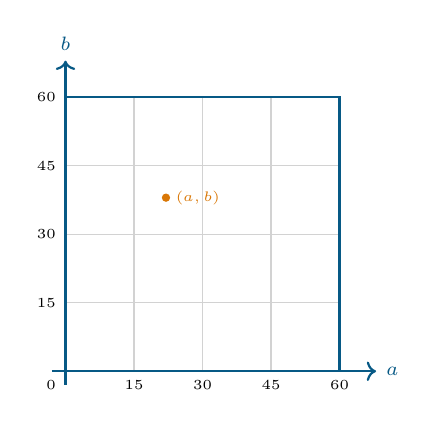
\begin{tikzpicture}[x=0.058cm,y=0.058cm]
\draw[gray!35,step=15] (0,0) grid (60,60);
\draw[->,thick,mainc] (-3,0)--(68,0) node[right,font=\scriptsize]{$a$};
\draw[->,thick,mainc] (0,-3)--(0,68) node[above,font=\scriptsize]{$b$};
\draw[mainc,thick] (0,0) rectangle (60,60);
\foreach \q in {15,30,45,60}{\node[font=\tiny,below] at (\q,0) {$\q$}; \node[font=\tiny,left] at (0,\q) {$\q$};}
\node[font=\tiny,below left] at (0,0) {$0$};
\fill[warmc] (22,38) circle (1.5pt) node[right,font=\tiny]{$(a,b)$};
\end{tikzpicture}}}{\pil{$\dfrac{11}{36}$}{$\dfrac5{12}$}{$\dfrac{31}{72}$}{$\dfrac7{16}$}{$\dfrac59$}}

% =====================================================================
\Needspace{16\baselineskip}
\bagian{B. Isian Singkat}{5 soal $\times$ 4 poin = 20 poin. Tuliskan hanya jawaban akhir.}

\tingkat{Tingkat Sedang}{soal 1 dan 2}
\soal{\gbr{Nilai ujian $800$ siswa berdistribusi normal. Menurut aturan empiris, $95\%$ siswa memperoleh nilai antara $58$ dan $82$ (daerah berarsir pada gambar). Banyak siswa yang nilainya \textbf{lebih dari $76$} kira-kira \dots.}{%
\begin{tikzpicture}[x=0.55cm,y=0.6cm]
\shadearea{skyl}{-2}{2}
\bellcurve
\draw[warmc,very thick,dashed] (1,0)--(1,{bell(1)});
\node[font=\scriptsize,below] at (-2,0) {58};
\node[font=\scriptsize,below] at (2,0) {82};
\node[font=\scriptsize\bfseries,warmc!70!black,below] at (1,0) {76};
\node[font=\scriptsize] at (-0.4,0.6) {$95\%$};
\end{tikzpicture}}}{\jwb}
\soal{\gbr{Dua dadu seimbang dilempar bersamaan. Misalkan $X$ adalah selisih mutlak kedua mata dadu; tabel pada gambar menunjukkan nilai $X$ untuk setiap pasangan hasil. Nilai harapan $E(X)$ adalah \dots\ (tulis sebagai pecahan paling sederhana).}{%
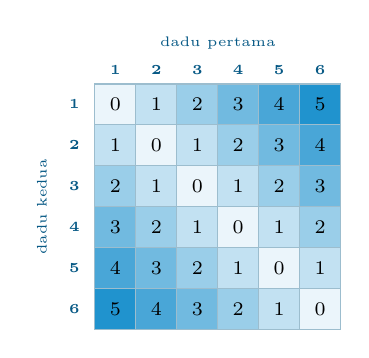
\begin{tikzpicture}[x=0.52cm,y=0.52cm]
\foreach \ia in {1,...,6}{
 \node[font=\tiny\bfseries,mainc] at (\ia,6.85) {\ia};
 \node[font=\tiny\bfseries,mainc] at (0,7-\ia) {\ia};
 \foreach \ib in {1,...,6}{
  \pgfmathtruncatemacro{\df}{abs(\ia-\ib)}
  \pgfmathtruncatemacro{\pc}{8+16*\df}
  \node[draw=mainc!40,fill=accc!\pc,minimum size=0.52cm,inner sep=0pt,font=\scriptsize] at (\ia,7-\ib) {\df};}}
\node[font=\tiny,mainc] at (3.5,7.5) {dadu pertama};
\node[font=\tiny,mainc,rotate=90] at (-0.8,3.5) {dadu kedua};
\end{tikzpicture}}}{\jwb}

\tingkat{Tingkat Sulit}{soal 3 sampai 5}
\soal{Variabel acak $X$ berdistribusi binomial $B(9,p)$ dengan $P(X=3)=P(X=4)$. Variansi $X$ adalah \dots\ (tulis sebagai desimal).}{\jwb}
\soal{\gbr{Titik $P$ dipilih secara acak (seragam) pada ruas garis $AB$ yang panjangnya $12$ cm. Peluang luas persegi panjang dengan panjang sisi $AP$ dan $PB$ \textbf{lebih dari $20$ cm$^2$} adalah \dots.}{%
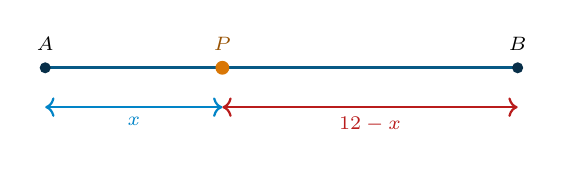
\begin{tikzpicture}[x=0.5cm]
\draw[mainc,very thick] (0,0)--(12,0);
\fill[deepc] (0,0) circle (2pt) (12,0) circle (2pt);
\fill[warmc] (4.5,0) circle (2.5pt);
\node[font=\scriptsize\bfseries,above] at (0,0.1) {$A$};
\node[font=\scriptsize\bfseries,above] at (12,0.1) {$B$};
\node[font=\scriptsize\bfseries,above,warmc!70!black] at (4.5,0.1) {$P$};
\draw[<->,accc,thick] (0,-0.5)--(4.5,-0.5) node[midway,below,font=\scriptsize]{$x$};
\draw[<->,brick,thick] (4.5,-0.5)--(12,-0.5) node[midway,below,font=\scriptsize]{$12-x$};
\end{tikzpicture}}}{\jwb}
\soal{Isi botol sirup berdistribusi normal dengan rata-rata $500$ ml dan simpangan baku $10$ ml. Botol layak jual jika isinya antara $480$ ml dan $520$ ml. Tiga botol diambil secara acak dan saling bebas. Dengan aturan empiris, peluang \textbf{tepat dua} botol layak jual adalah \dots\ (bulatkan sampai tiga angka di belakang koma).}{\jwb}

% =====================================================================
\Needspace{16\baselineskip}
\bagian{C. Uraian (Essay)}{5 soal $\times$ 8 poin = 40 poin. Tuliskan langkah penyelesaian dengan lengkap.}

\tingkat{Tingkat Sedang}{soal 1 dan 2}
\soal{\gbr{Sebuah wahana permainan memakai roda putar yang terbagi menjadi empat sektor (lihat gambar). Pemain memutar roda sekali dan menerima hadiah sesuai sektor tempat roda berhenti. Misalkan $X$ adalah hadiah dalam ribu rupiah. Sudut sektor Rp0, Rp2.000, dan Rp4.000 berturut-turut adalah $180^\circ$, $90^\circ$, dan $45^\circ$.\par\smallskip
(a) Tentukan sudut sektor Rp8.000, lalu buat tabel distribusi peluang $X$.\par
(b) Hitung nilai harapan $E(X)$.\par
(c) Hitung $\Var(X)$ dan simpangan baku $X$ (bentuk akar boleh).\par
(d) Penyelenggara menarik biaya Rp2.500 per putaran. Berapa keuntungan harapan penyelenggara dari $400$ putaran? Jelaskan arti nilai harapan tersebut.}{%
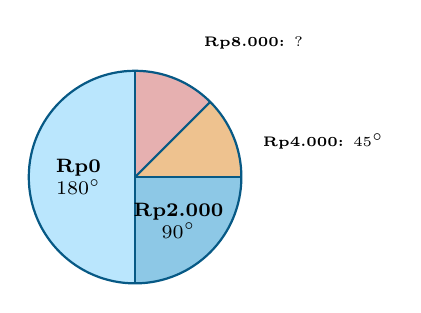
\begin{tikzpicture}
\def\R{1.35}
\fill[skyl] (0,0) -- (90:\R) arc (90:270:\R) -- cycle;
\fill[accc!45] (0,0) -- (270:\R) arc (270:360:\R) -- cycle;
\fill[warmc!45] (0,0) -- (0:\R) arc (0:45:\R) -- cycle;
\fill[brick!35] (0,0) -- (45:\R) arc (45:90:\R) -- cycle;
\draw[mainc,thick] (0,0) circle (\R);
\foreach \an in {0,45,90,270}{\draw[mainc,thick] (0,0)--(\an:\R);}
\node[font=\scriptsize\bfseries,align=center] at (180:0.72) {Rp0\\$180^\circ$};
\node[font=\scriptsize\bfseries,align=center] at (315:0.78) {Rp2.000\\$90^\circ$};
\node[font=\tiny\bfseries,anchor=west] at (1.5,0.45) {Rp4.000: $45^\circ$};
\node[font=\tiny\bfseries,anchor=south west] at (0.75,1.5) {Rp8.000: $?$};
\end{tikzpicture}}}{\poin{8}}
\soal{\gbr{Sebuah tim voli menang pada setiap pertandingan dengan peluang $0{,}6$, dan hasil antarpertandingan saling bebas. Dalam sebuah turnamen, tim itu bermain $4$ pertandingan. Misalkan $X$ adalah banyak kemenangan; diagram batang distribusi $X$ ditunjukkan pada gambar.\par\smallskip
(a) Hitung $P(X=k)$ untuk $k=0,1,2,3,4$ dan sajikan dalam tabel.\par
(b) Tim lolos ke babak berikutnya jika menang paling sedikit $3$ pertandingan. Hitung peluang tim lolos.\par
(c) Hitung $E(X)$ dan $\Var(X)$.\par
(d) Pada gambar terlihat dua batang tertinggi sama tinggi. Tentukan modusnya, lalu jelaskan dengan membandingkan $\dfrac{P(X=k+1)}{P(X=k)}$ mengapa hal itu terjadi.}{%
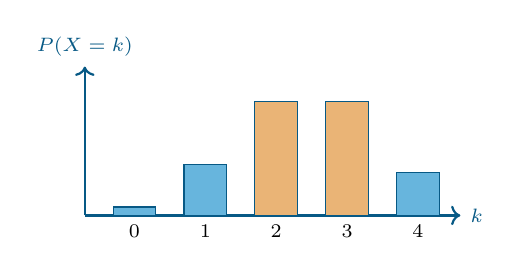
\begin{tikzpicture}[x=0.9cm,y=4.2cm]
\draw[->,thick,mainc] (-0.2,0)--(5.1,0) node[right,font=\scriptsize]{$k$};
\draw[->,thick,mainc] (-0.2,0)--(-0.2,0.45) node[above,font=\scriptsize]{$P(X=k)$};
\foreach \ix/\hh in {0/0.0256,1/0.1536,2/0.3456,3/0.3456,4/0.1296}{
 \ifnum\ix=2 \def\cl{warmc!55}\else\ifnum\ix=3 \def\cl{warmc!55}\else\def\cl{accc!60}\fi\fi
 \fill[\cl] (\ix+0.2,0) rectangle (\ix+0.8,\hh);
 \draw[mainc] (\ix+0.2,0) rectangle (\ix+0.8,\hh);
 \node[font=\scriptsize,below] at (\ix+0.5,0) {$\ix$};}
\end{tikzpicture}}}{\poin{8}}

\Needspace{22\baselineskip}
\tingkat{Tingkat Sulit}{soal 3 dan 4}
\soal{\gbr{Umur sebuah lampu produksi mesin lama berdistribusi normal dengan rata-rata $1.000$ jam dan simpangan baku $100$ jam.\par\smallskip
(a) Produsen menetapkan masa garansi sehingga $2{,}28\%$ lampu rusak sebelum garansi berakhir. Tentukan masa garansi tersebut.\par
(b) Dari pengiriman $5.000$ lampu mesin lama, perkirakan banyak lampu yang umurnya antara $900$ dan $1.150$ jam.\par
(c) Mesin baru menghasilkan umur lampu yang juga normal dengan rata-rata tetap $1.000$ jam tetapi simpangan baku lebih kecil. Dengan masa garansi yang sama seperti pada (a), hanya $0{,}62\%$ lampu rusak dalam masa garansi. Tentukan simpangan baku mesin baru.\par
(d) Lampu A dari mesin lama berumur $1.200$ jam dan lampu B dari mesin baru berumur $1.160$ jam. Lampu mana yang lebih istimewa dibandingkan lampu-lampu produksi mesinnya sendiri? Jelaskan dengan skor $z$.}{%
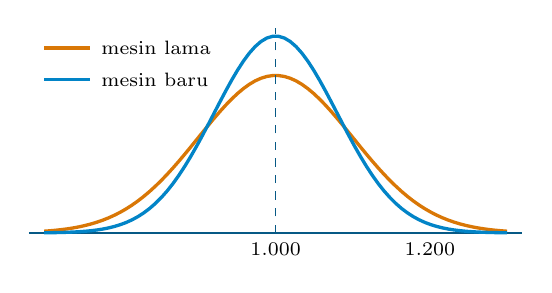
\begin{tikzpicture}[x=0.0098cm,y=1cm]
\draw[thick,mainc] (-320,0)--(320,0);
\draw[warmc,very thick,domain=700:1300,samples=80] plot ({\x-1000},{2.0*exp(-0.5*((\x-1000)/100)^2)});
\draw[accc,very thick,domain=700:1300,samples=80] plot ({\x-1000},{2.5*exp(-0.5*((\x-1000)/80)^2)});
\draw[dashed,mainc] (0,0)--(0,2.6);
\node[font=\scriptsize,below] at (0,0) {$1.000$};
\node[font=\scriptsize,below] at (200,0) {$1.200$};
\draw[warmc,very thick] (-300,2.35)--(-240,2.35) node[right,font=\scriptsize,black]{mesin lama};
\draw[accc,very thick] (-300,1.95)--(-240,1.95) node[right,font=\scriptsize,black]{mesin baru};
\end{tikzpicture}}}{\poin{8}}
\soal{\gbr{Seorang pecinta teh mengaku dapat membedakan teh merek P dan merek Q lewat rasa. Dalam uji buta, ia menebak merek pada $100$ cangkir yang disajikan acak. Misalkan $X$ banyak tebakan yang benar. Jika ia sebenarnya hanya menebak, maka $X\sim B(100;0{,}5)$.\par\smallskip
(a) Hitung $\mu=np$ dan $\sigma$, lalu tunjukkan bahwa pendekatan normal layak dipakai.\par
(b) Ia benar pada $58$ cangkir. Dengan pendekatan normal dan koreksi kontinuitas, hitung peluang memperoleh hasil sebaik itu atau lebih baik, yaitu $P(X\ge58)$, jika ia hanya menebak.\par
(c) Panitia mengakui kemampuannya hanya jika peluang memperoleh hasil sebaik itu secara kebetulan paling besar $2{,}28\%$. Tentukan banyak tebakan benar minimum agar kemampuannya diakui.\par
(d) Apakah $58$ tebakan benar cukup meyakinkan panitia? Tafsirkan hasilnya dan jelaskan mengapa kegagalan itu belum membuktikan bahwa ia hanya menebak.}{%
\begin{tikzpicture}[x=0.55cm,y=0.6cm]
\shadearea{brick!45}{1.5}{3.4}
\bellcurve
\draw[dashed,mainc] (1.5,0)--(1.5,{bell(1.5)});
\node[font=\scriptsize,below] at (-2,0) {40};
\node[font=\scriptsize,below] at (0,0) {50};
\node[font=\scriptsize\bfseries,brick,below] at (1.5,0) {57,5};
\node[font=\tiny,brick] at (2.8,0.8) {$P(X\ge58)$};
\node[font=\scriptsize,mainc] at (0,0.6) {$B(100;0{,}5)$};
\end{tikzpicture}}}{\poin{8}}

\Needspace{26\baselineskip}
\tingkat{Tingkat HOTS}{soal 5}
\soal{\gbr{Sebuah pesawat nirawak memakai beberapa mesin identik. Setiap mesin berfungsi dengan peluang $p$ dan berfungsi atau tidaknya mesin saling bebas. Ada dua rancangan. \textbf{Rancangan A}: $3$ mesin, pesawat berfungsi jika \emph{minimal $2$} mesin berfungsi. \textbf{Rancangan B}: $5$ mesin, pesawat berfungsi jika \emph{minimal $3$} mesin berfungsi. Keandalan rancangan adalah peluang pesawat berfungsi, ditulis $R_A(p)$ dan $R_B(p)$. Gambar menunjukkan grafik keduanya (garis putus-putus: satu mesin tunggal, $R=p$).\par\smallskip
(a) Tunjukkan $R_A(p)=3p^2-2p^3$, lalu hitung $R_A(0{,}8)$.\par
(b) Tunjukkan $R_B(p)=10p^3-15p^4+6p^5$, lalu hitung $R_B(0{,}8)$.\par
(c) Buktikan bahwa $R_B(p)-R_A(p)=3p^2(1-p)^2(2p-1)$.\par
(d) Berdasarkan (c), tentukan untuk nilai $p$ berapa rancangan B lebih andal, dan kaitkan dengan titik potong pada gambar. Jika mesin yang tersedia hanya berpeluang berfungsi $p=0{,}4$, rancangan mana yang sebaiknya dipilih? Hitung selisih keandalannya.}{%
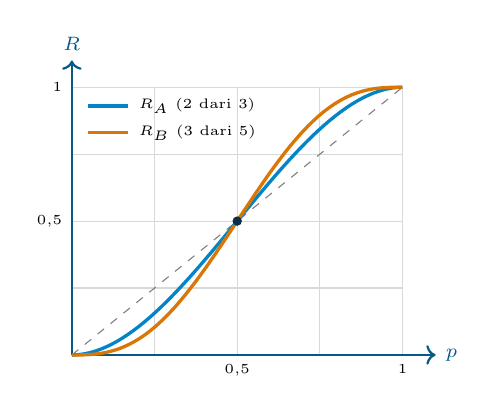
\begin{tikzpicture}[x=4.2cm,y=3.4cm]
\draw[gray!30,xstep=0.25,ystep=0.25] (0,0) grid (1,1);
\draw[->,thick,mainc] (0,0)--(1.1,0) node[right,font=\scriptsize]{$p$};
\draw[->,thick,mainc] (0,0)--(0,1.1) node[above,font=\scriptsize]{$R$};
\draw[gray,dashed] (0,0)--(1,1);
\draw[accc,very thick,domain=0:1,samples=60] plot (\x,{3*\x*\x-2*\x*\x*\x});
\draw[warmc,very thick,domain=0:1,samples=60] plot (\x,{10*\x^3-15*\x^4+6*\x^5});
\fill[deepc] (0.5,0.5) circle (1.7pt);
\foreach \q/\lab in {0.5/{0{,}5},1/{1}}{\node[font=\tiny,below] at (\q,0) {$\lab$}; \node[font=\tiny,left] at (0,\q) {$\lab$};}
\draw[accc,very thick] (0.05,0.93)--(0.17,0.93) node[right,font=\tiny,black]{$R_A$ (2 dari 3)};
\draw[warmc,very thick] (0.05,0.83)--(0.17,0.83) node[right,font=\tiny,black]{$R_B$ (3 dari 5)};
\end{tikzpicture}}}{\poin{8}}

% =====================================================================
\newpage
\bagian{Kunci Jawaban dan Pembahasan Singkat}{Untuk guru dan pembahasan mandiri}
\par\vspace{0.6em}{\bfseries\color{mainc}Kunci Pilihan Ganda}\par\vspace{0.3em}
\small
\begin{tabularx}{\linewidth}{@{}*{10}{>{\centering\arraybackslash}X}@{}}\hline \textbf{1} & \textbf{2} & \textbf{3} & \textbf{4} & \textbf{5} & \textbf{6} & \textbf{7} & \textbf{8} & \textbf{9} & \textbf{10}\\ \hline B & D & C & A & E & D & A & A & E & B\\ \hline\end{tabularx}\\[6pt]
\begin{tabularx}{\linewidth}{@{}*{10}{>{\centering\arraybackslash}X}@{}}\hline \textbf{11} & \textbf{12} & \textbf{13} & \textbf{14} & \textbf{15} & \textbf{16} & \textbf{17} & \textbf{18} & \textbf{19} & \textbf{20}\\ \hline D & E & B & E & D & C & C & B & A & C\\ \hline\end{tabularx}
\par\vspace{0.4em}{\bfseries\color{mainc}Kunci Isian Singkat:}\ \ 1) $128$\quad 2) $\dfrac{35}{18}$\quad 3) $2{,}16$\quad 4) $\dfrac23$\quad 5) $0{,}135$
\par\vspace{0.8em}{\bfseries\color{mainc}\normalsize Pembahasan Pilihan Ganda}\par\vspace{0.2em}
\small\begin{enumerate}[leftmargin=2em,itemsep=2pt,topsep=2pt]
\item[\textbf{1.}] \textbf{(B)} Jumlah peluang $1$: $0{,}1+0{,}4+k+0{,}2=1$, sehingga $k=0{,}3$. $E(X)=0(0{,}1)+1(0{,}4)+2(0{,}3)+3(0{,}2)=0{,}4+0{,}6+0{,}6=1{,}6$. (Jebakan: mengabaikan $k$ menghasilkan $1{,}0$.)
\item[\textbf{2.}] \textbf{(D)} Kelipatan $6$: $6,12,\dots,36$ ada $6$ bilangan. Kelipatan $8$: $8,16,\dots,40$ ada $5$ bilangan. Kelipatan keduanya (kelipatan $24$): hanya $24$, ada $1$ bilangan. Banyak bilangan yang memenuhi $6+5-1=10$, sehingga peluangnya $\frac{10}{40}=\frac14$. (Jebakan: tidak mengurangi irisan menghasilkan $\frac{11}{40}$.)
\item[\textbf{3.}] \textbf{(C)} $X\sim B(3;0{,}7)$: $P(X=2)=\binom32(0{,}7)^2(0{,}3)=3\cdot0{,}49\cdot0{,}3=0{,}441$. (Jebakan: $0{,}784$ adalah peluang \emph{paling sedikit} dua.)
\item[\textbf{4.}] \textbf{(A)} $z=\frac{26-30}{2}=-2$, yaitu $\mu-2\sigma$. Menurut aturan empiris, $95\%$ data berada di dalam $\mu\pm2\sigma$, sehingga $5\%$ di luar dan terbagi sama di dua ekor: $2{,}5\%$ di tiap ekor.
\item[\textbf{5.}] \textbf{(E)} (i) Kurva normal simetris terhadap $\mu$ dan puncaknya di $\mu$, jadi \textbf{B}. (ii) $E(X)=10(0{,}3)=3$ dan $\Var(X)=10(0{,}3)(0{,}7)=2{,}1$, jadi \textbf{B}. (iii) Pada distribusi kontinu, peluang satu nilai tepat sama dengan $0$, sehingga $P(X=5)=0$, jadi \textbf{S}. Urutan: B, B, S.
\item[\textbf{6.}] \textbf{(D)} Setelah diketahui $X>30$, ruang sampel menyusut menjadi selang $(30,120]$ yang panjangnya $90$. Kejadian $30<X\le90$ panjangnya $60$. Peluangnya $\frac{60}{90}=\frac23$. (Jebakan: tanpa memakai syarat diperoleh $\frac{60}{120}=\frac12$.)
\item[\textbf{7.}] \textbf{(A)} $X\sim B(4;0{,}8)$. $P(X\le2)=1-P(X=3)-P(X=4)=1-\left[4(0{,}8)^3(0{,}2)+(0{,}8)^4\right]=1-[0{,}4096+0{,}4096]=0{,}1808$. Cek: $0{,}0016+0{,}0256+0{,}1536=0{,}1808$.
\item[\textbf{8.}] \textbf{(A)} $78=\mu+1{,}5\sigma$ dan $66=\mu-0{,}5\sigma$. Dikurangkan: $12=2\sigma$, sehingga $\sigma=6$ dan $\mu=69$. $P(X>75)$: $z=\frac{75-69}{6}=1$, jadi $1-\Phi(1)=1-0{,}8413=0{,}1587$.
\item[\textbf{9.}] \textbf{(E)} Peluang tiap nilai adalah selisih nilai $F$ berurutan: $P(0)=0{,}15$; $P(1)=0{,}40-0{,}15=0{,}25$; $P(2)=0{,}75-0{,}40=0{,}35$; $P(3)=1-0{,}75=0{,}25$. $E(X)=0+0{,}25+0{,}70+0{,}75=1{,}70$.
\item[\textbf{10.}] \textbf{(B)} $E(X)=np$ dan $\Var(X)=np(1-p)$. Dari $np=2np(1-p)$ diperoleh $1-p=\frac12$, jadi $p=\frac12$. Lalu $p^n=\left(\frac12\right)^n=\frac1{64}$ memberi $n=6$. $P(X\ge5)=\frac{\binom65+\binom66}{64}=\frac{6+1}{64}=\frac7{64}$.
\item[\textbf{11.}] \textbf{(D)} $0{,}0668=1-0{,}9332=1-\Phi(1{,}5)=\Phi(-1{,}5)$, sehingga batas bawah daerah arsiran berada di $z=-1{,}5$. Maka $k=72-1{,}5(8)=60$. (Jebakan: memakai $+1{,}5$ menghasilkan $84$.)
\item[\textbf{12.}] \textbf{(E)} $X\sim B(4;\frac12)$: $E(X)=2$, $\Var(X)=1$, sehingga $E(X^2)=\Var(X)+[E(X)]^2=1+4=5$. Hadiah rata-rata $5$ ribu rupiah, yaitu Rp5.000. Hasil rata-rata pemain $5.000-6.000=-1.000$, jadi rugi Rp1.000. Cek langsung: $\frac{0\cdot1+1\cdot4+4\cdot6+9\cdot4+16\cdot1}{16}=\frac{80}{16}=5$. (Jebakan: memakai $[E(X)]^2=4$ menghasilkan rugi Rp2.000.)
\item[\textbf{13.}] \textbf{(B)} $15{,}87\%=\Phi(-1)$ berarti $40=\mu-\sigma$. $2{,}28\%=1-\Phi(2)$ berarti $70=\mu+2\sigma$. Dikurangkan: $30=3\sigma$, sehingga $\sigma=10$ dan $\mu=50$. $P(45<X<65)=P(-0{,}5<Z<1{,}5)=\Phi(1{,}5)-\Phi(-0{,}5)=0{,}9332-(1-0{,}6915)=0{,}9332-0{,}3085=0{,}6247$.
\item[\textbf{14.}] \textbf{(E)} $P(X=0)=(1-p)^4=\frac{16}{81}$ sehingga $1-p=\frac23$ dan $p=\frac13$. $P(X=1)=4\cdot\frac13\cdot\left(\frac23\right)^3=\frac{32}{81}$. $P(X\le1)=\frac{16+32}{81}=\frac{48}{81}=\frac{16}{27}$.
\item[\textbf{15.}] \textbf{(D)} Perbandingan peluang berurutan: $\frac{P(X=k+1)}{P(X=k)}=\frac{20-k}{k+1}\cdot\frac{0{,}3}{0{,}7}=\frac{3(20-k)}{7(k+1)}$. Peluang naik selama rasio $>1$, yaitu $60-3k>7k+7$, atau $k<5{,}3$. Jadi $P(5)<P(6)$ (rasio $\frac{45}{42}>1$) dan $P(6)>P(7)$ (rasio $\frac{42}{49}<1$). Modus $x=6$ (sama dengan $\lfloor(n+1)p\rfloor=\lfloor6{,}3\rfloor$).
\item[\textbf{16.}] \textbf{(C)} Peluang paling sedikit satu gambar $=1-\frac1{32}=\frac{31}{32}$. Peluang tepat dua gambar $=\frac{\binom52}{32}=\frac{10}{32}$ (kejadian ini sudah termasuk dalam syarat). Peluang bersyarat $=\frac{10/32}{31/32}=\frac{10}{31}$. (Jebakan: mengabaikan syarat menghasilkan $\frac5{16}$.)
\item[\textbf{17.}] \textbf{(C)} Transformasi linear dengan $a>0$ mempertahankan bentuk normal, sehingga $Y\sim N(70,9^2)$ (di sini $a=\frac34$, $b=25$, tetapi nilai ini tidak diperlukan). $z=\frac{79-70}{9}=1$, $P(Y>79)=1-0{,}8413=0{,}1587$. Banyak siswa $500\times0{,}1587\approx79{,}33\approx79$. (Jebakan: $421$ adalah banyak siswa dengan nilai di bawah $79$.)
\item[\textbf{18.}] \textbf{(B)} Akar real jika diskriminan $\ge0$: $4X^2-4(X+6)\ge0\Rightarrow X^2-X-6\ge0\Rightarrow(X-3)(X+2)\ge0$, yaitu $X\le-2$ atau $X\ge3$. Dalam $[-3,6]$: selang $[-3,-2]$ panjang $1$ dan $[3,6]$ panjang $3$. Peluang $=\frac{1+3}{9}=\frac49$. (Jebakan: hanya memakai $X\ge3$ menghasilkan $\frac13$.)
\item[\textbf{19.}] \textbf{(A)} Pernyataan (1): misalkan $L=b-a$. $P(X<6)=\frac{6-a}{L}=\frac14$ memberi $a=6-\frac L4$, dan $P(X>9)=\frac{b-9}{L}=\frac12$ memberi $b=9+\frac L2$. Maka $L=b-a=3+\frac{3L}{4}$, sehingga $L=12$, $a=3$, $b=15$. Jadi $P(X<7)=\frac{7-3}{12}=\frac13$: cukup. Pernyataan (2): $\frac{(b-a)^2}{12}=12$ hanya memberi $b-a=12$, letak selang tidak diketahui, jadi tidak cukup. Jawaban A.
\item[\textbf{20.}] \textbf{(C)} Tidak bertemu jika (i) Andi tiba lebih dulu dan $b-a>20$: segitiga siku-siku dengan sisi $60-20=40$, luas $\frac12\cdot40\cdot40=800$; atau (ii) Bimo tiba lebih dulu dan $a-b>10$: sisi $60-10=50$, luas $\frac12\cdot50\cdot50=1.250$. Luas tidak bertemu $=2.050$ dari $3.600$. Peluang bertemu $=1-\frac{2.050}{3.600}=\frac{1.550}{3.600}=\frac{31}{72}$. (Jebakan: jika keduanya menunggu $15$ menit, hasilnya $\frac7{16}$.)
\end{enumerate}
\par\Needspace{6\baselineskip}\vspace{0.6em}{\bfseries\color{mainc}\normalsize Pembahasan Isian Singkat}\par\vspace{0.2em}
\small\begin{enumerate}[leftmargin=2em,itemsep=2pt,topsep=2pt]
\item[\textbf{1.}] \textbf{Jawaban: $128$.} $95\%$ data berada di $\mu\pm2\sigma$: $\mu=\frac{58+82}{2}=70$ dan $2\sigma=12$, jadi $\sigma=6$. Nilai $76=\mu+\sigma$. Menurut aturan empiris, $P(X>\mu+\sigma)=\frac{100\%-68\%}{2}=16\%$. Banyak siswa $800\times0{,}16=128$.
\item[\textbf{2.}] \textbf{Jawaban: $\dfrac{35}{18}$.} Dari tabel $6\times6$: selisih $0$ ada $6$ sel, selisih $1$ ada $10$, selisih $2$ ada $8$, selisih $3$ ada $6$, selisih $4$ ada $4$, selisih $5$ ada $2$ (jumlah $36$). $E(X)=\frac{0\cdot6+1\cdot10+2\cdot8+3\cdot6+4\cdot4+5\cdot2}{36}=\frac{70}{36}=\frac{35}{18}$.
\item[\textbf{3.}] \textbf{Jawaban: $2{,}16$.} $\binom93p^3(1-p)^6=\binom94p^4(1-p)^5\Rightarrow84(1-p)=126p\Rightarrow p=\frac25$. $\Var(X)=9\cdot\frac25\cdot\frac35=\frac{54}{25}=2{,}16$.
\item[\textbf{4.}] \textbf{Jawaban: $\dfrac23$.} Misalkan $AP=x$, maka $PB=12-x$ dan luas $x(12-x)>20$, yaitu $x^2-12x+20<0$, atau $(x-2)(x-10)<0$, sehingga $2<x<10$. Panjang selang $8$ dari $12$: peluang $\frac{8}{12}=\frac23$.
\item[\textbf{5.}] \textbf{Jawaban: $0{,}135$.} Selang $480$ sampai $520$ adalah $\mu\pm2\sigma$, jadi peluang botol layak $0{,}95$. Banyak botol layak dari $3$ botol berdistribusi $B(3;0{,}95)$: $P(\text{tepat }2)=\binom32(0{,}95)^2(0{,}05)=3\cdot0{,}9025\cdot0{,}05=0{,}135375\approx0{,}135$.
\end{enumerate}
\par\Needspace{8\baselineskip}\vspace{0.6em}{\bfseries\color{mainc}\normalsize Pembahasan dan Pedoman Penskoran Uraian}\par\vspace{0.2em}
\small\begin{enumerate}[leftmargin=2em,itemsep=3pt,topsep=2pt]
\item[\textbf{1.}] (a) Sudut sektor Rp8.000 $=360^\circ-(180^\circ+90^\circ+45^\circ)=45^\circ$. Peluang tiap sektor $=\frac{\text{sudut}}{360^\circ}$. Tabel: $x=0,2,4,8$ dengan $P(X=x)=\frac12,\frac14,\frac18,\frac18$ (jumlah $1$). (b) $E(X)=0\cdot\frac12+2\cdot\frac14+4\cdot\frac18+8\cdot\frac18=0+0{,}5+0{,}5+1=2$ ribu rupiah, yaitu Rp2.000. (c) $E(X^2)=0+4\cdot\frac14+16\cdot\frac18+64\cdot\frac18=1+2+8=11$. $\Var(X)=11-2^2=7$ dan simpangan baku $\sqrt7\approx2{,}65$ ribu rupiah. (d) Keuntungan harapan per putaran $2.500-2.000=500$ rupiah, sehingga untuk $400$ putaran $400\times500=$ Rp200.000. Nilai harapan adalah rata-rata hadiah dalam jangka panjang: pada satu putaran pemain bisa menang Rp8.000 (melebihi biaya), tetapi rata-rata penyelenggara tetap untung. \\ \textit{Penskoran: tiap bagian 2 poin.}
\item[\textbf{2.}] (a) $P(0)=(0{,}4)^4=0{,}0256$; $P(1)=4(0{,}6)(0{,}4)^3=0{,}1536$; $P(2)=6(0{,}6)^2(0{,}4)^2=0{,}3456$; $P(3)=4(0{,}6)^3(0{,}4)=0{,}3456$; $P(4)=(0{,}6)^4=0{,}1296$ (jumlah $1$). (b) $P(X\ge3)=0{,}3456+0{,}1296=0{,}4752$. (c) $E(X)=4(0{,}6)=2{,}4$ dan $\Var(X)=4(0{,}6)(0{,}4)=0{,}96$. (d) $\frac{P(X=k+1)}{P(X=k)}=\frac{4-k}{k+1}\cdot\frac{0{,}6}{0{,}4}=\frac{3(4-k)}{2(k+1)}$. Untuk $k=2$ rasio $=\frac{3\cdot2}{2\cdot3}=1$, jadi $P(2)=P(3)$. Untuk $k=1$ rasio $2{,}25>1$ (naik) dan untuk $k=3$ rasio $0{,}375<1$ (turun). Modusnya $2$ dan $3$ (dua modus), terjadi karena $(n+1)p=5(0{,}6)=3$ bilangan bulat. \\ \textit{Penskoran: tiap bagian 2 poin.}
\item[\textbf{3.}] (a) $P(X<k)=0{,}0228=1-\Phi(2)=\Phi(-2)$, sehingga $z=-2$ dan $k=1.000-2(100)=800$ jam. (b) $z_1=\frac{900-1.000}{100}=-1$ dan $z_2=\frac{1.150-1.000}{100}=1{,}5$. $P=\Phi(1{,}5)-\Phi(-1)=0{,}9332-0{,}1587=0{,}7745$. Banyak lampu $5.000\times0{,}7745=3.872{,}5\approx3.873$. (c) $P(Y<800)=0{,}0062=1-\Phi(2{,}5)=\Phi(-2{,}5)$, sehingga $\frac{800-1.000}{\sigma}=-2{,}5$ dan $\sigma=80$ jam. (d) Lampu A: $z=\frac{1.200-1.000}{100}=2$. Lampu B: $z=\frac{1.160-1.000}{80}=2$. Skor $z$ sama, jadi keduanya sama istimewa: masing-masing berada $2$ simpangan baku di atas rata-rata mesinnya (sekitar $2{,}28\%$ teratas). Selisih umur mentah ($200$ jam dan $160$ jam) tidak dapat dibandingkan langsung karena sebaran kedua mesin berbeda. \\ \textit{Penskoran: tiap bagian 2 poin.}
\item[\textbf{4.}] (a) $\mu=np=100(0{,}5)=50$ dan $\sigma=\sqrt{100(0{,}5)(0{,}5)}=5$. Syarat $np=50\ge5$ dan $n(1-p)=50\ge5$ terpenuhi, jadi $B(100;0{,}5)\approx N(50,5^2)$. (b) Dengan koreksi kontinuitas $X\ge58$ menjadi $X\ge57{,}5$: $z=\frac{57{,}5-50}{5}=1{,}5$, $P=1-\Phi(1{,}5)=1-0{,}9332=0{,}0668$ (sekitar $6{,}68\%$). (c) Perlu $P(X\ge k)\le0{,}0228=1-\Phi(2)$, yaitu $\frac{(k-0{,}5)-50}{5}\ge2$, sehingga $k\ge60{,}5$ dan $k$ minimum $=61$. (Untuk $k=60$ diperoleh $z=1{,}9<2$, peluangnya masih lebih dari $2{,}28\%$.) (d) $58<61$ dan peluang kebetulan $6{,}68\%>2{,}28\%$, jadi hasil itu belum cukup meyakinkan panitia. Namun ini hanya berarti bukti belum cukup kuat, bukan bukti bahwa ia pasti menebak: orang yang sedikit mampu membedakan pun bisa memperoleh $58$ benar, dan jumlah cangkir yang lebih banyak akan membuat uji lebih tajam. \\ \textit{Penskoran: (a) 1 poin; (b) 2 poin; (c) 3 poin; (d) 2 poin.}
\item[\textbf{5.}] (a) Pesawat A berfungsi jika tepat $2$ atau semua $3$ mesin berfungsi: $R_A=\binom32p^2(1-p)+p^3=3p^2-3p^3+p^3=3p^2-2p^3$. $R_A(0{,}8)=3(0{,}64)-2(0{,}512)=1{,}92-1{,}024=0{,}896$. (b) $R_B=\binom53p^3(1-p)^2+\binom54p^4(1-p)+p^5=10p^3(1-2p+p^2)+5p^4-5p^5+p^5=10p^3-15p^4+6p^5$. $R_B(0{,}8)=10(0{,}512)-15(0{,}4096)+6(0{,}32768)=5{,}12-6{,}144+1{,}96608=0{,}94208$. (c) $R_B-R_A=-3p^2+12p^3-15p^4+6p^5=-3p^2(1-4p+5p^2-2p^3)$. Karena $(1-p)^2(1-2p)=1-4p+5p^2-2p^3$, maka $R_B-R_A=-3p^2(1-p)^2(1-2p)=3p^2(1-p)^2(2p-1)$. (Cek di $p=0{,}8$: $3(0{,}64)(0{,}04)(0{,}6)=0{,}04608=0{,}94208-0{,}896$.) (d) Untuk $0<p<1$ faktor $3p^2(1-p)^2>0$, sehingga tanda selisih ditentukan oleh $2p-1$: B lebih andal jika $p>\frac12$, A lebih andal jika $p<\frac12$, dan keduanya sama ($0{,}5$) saat $p=\frac12$, yaitu titik potong kedua grafik. Untuk $p=0{,}4$: $R_A=3(0{,}16)-2(0{,}064)=0{,}352$ dan selisih $R_B-R_A=3(0{,}16)(0{,}36)(-0{,}2)=-0{,}03456$, sehingga $R_B=0{,}31744$. Pilih rancangan A. Menambah mesin hanya menguntungkan jika setiap mesin lebih banyak berfungsi daripada gagal. \\ \textit{Penskoran: (a) 2 poin; (b) 2 poin; (c) 2 poin; (d) 2 poin.}
\end{enumerate}
\end{document}
